	\سؤال{نصب سیستم‌عامل}

با توجه به صحبت‌های انجام‌شده نیازی به آوردن اسکرین‌شات‌های این قسمت نیست.

\سؤال{آشنایی با دستورات پایه‌ی لینوکس}
\begin{enumerate}
	\item 
		\textbf{دستور \lr{pwd}}
		
		\begin{code}
			> pwd
			
			/home/mostafa/Desktop/University/OS-Lab
		\end{code}
	\item 
		\textbf{دستور \lr{cd} و دستور \lr{mkdir}}
		\begin{code}
			> cd /tmp
			
			> mkdir oslab1
			
			> cd oslab1
		\end{code}
	\item 
		\textbf{دستور \lr{nano}}
		\begin{code}
			> sudo nano information.txt
		\end{code}
	
	\item 
		\textbf{دستور \lr{mv}}
		\begin{code}
			> sudo mv information.txt myinformation.txt
		\end{code}
	\item 
		\textbf{دستور \lr{cp}}
		
		\begin{code}
			> sudo cp information.txt backupinfo.txt
		\end{code}
	\item  
		\textbf{دستور \lr{cat}}
		\begin{code}
			> cat myinformation.txt
		\end{code}
	\item دستور «\lr{>}» تمام محتویات قبلی را پاک کرده و محتوای جدید را به فایل اضافه می‌کند. اصطلاحا به این کار «\lr{overwrite}» می‌گویند.
	 اما دستور «$>>$»، محتوای قبلی را نگه می‌دارد و محتوای جدید را به آخر محتوای قبلی اضافه می‌کند. اصطلاحا به این کار «append» می‌گویند.
	\item 
		\textbf{ساخت فایل جدید با دستور \lr{cat}}
		\begin{code}
			> cat > testfile.txt
		\end{code}
	\item 
		\textbf{لیست پردازه‌ها}
		\begin{code}
			> ps aux
		\end{code}
		\begin{figure}[!h]
			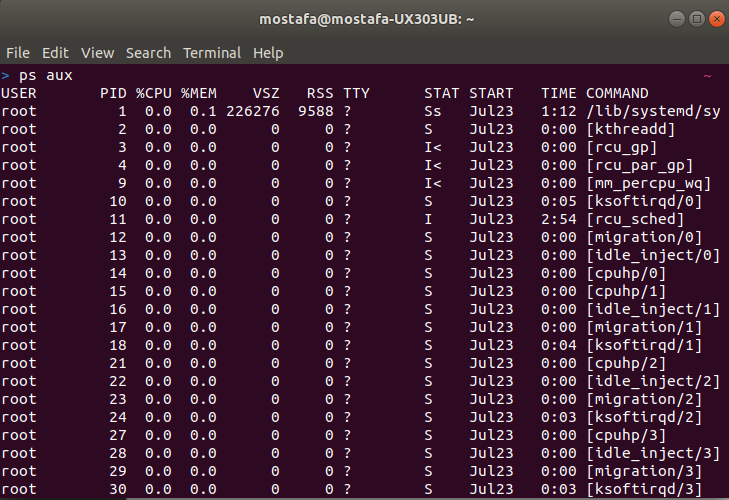
\includegraphics[width=\linewidth]{9.png}
			\caption{نمایش لیست پردازه‌ها با دستور \lr{ps}}
		\end{figure}
	\item 
		\textbf{دستور \lr{grep}}
		\begin{code}
			> ps aux | grep a
		\end{code}
	
	\item 
		\textbf{دستور \lr{ls}}
		\begin{code}
			> cd /usr/bin
			
			> ls
		\end{code}
	
	\item 
		\textbf{نمایش ججم و نام فایل‌ها}
		\begin{code}
			> ls -sh
		\end{code}
	\item 
		\textbf{جست‌وجو در نام فایل‌ها}
		\begin{code}
			> ls -h | grep 'id\textbackslash|fs'
		\end{code}
 
\end{enumerate}

\textbf{فعالیت}
\begin{itemize}
	\item 
		کاربرد دستورات
		
		\begin{itemize}
			\item دستور \lr{cut}: برای برش یا جدا کردن بخشی از هر خط از فایل و چاپ کردن نتیجه درون خروجی استاندارد، از این دستور استفاده می‌شود.
			\item دستور \lr{find}:
			از این دستور می‌توان برای پیدا کردن فایل‌ها و دایرکتوری‌ها و هم‌چنین انجام عملیات پی‌در‌پی روی آن‌ها استفاده می‌شود.
			\item دستور \lr{head}:
			همان‌طور که از نامش پیداست، (به صورت پیش‌فرض) ده خط اول از یک فایل را نشان می‌دهد. این تعداد خط را می‌توان تغییر داد.
			\item دستور \lr{tail}:
			همان‌طور که از نامش پیداست، (به‌صورت پیش‌فرض) ده خط آخر از یک فایل را نمایش می‌دهد. این تعداد خط را می‌توان تغییر داد.
			\item دستور \lr{touch}:
			دستور استاندارد سیستم‌عامل لینوکس برای ایجاد و تغییر \lr{timestamp} فایل است. از آن برای ایجاد یک فایل بدون محتوا نیز استفاده می‌شود.
			
			\item دستور \lr{wc}:
			از این دستور برای شمارش تعداد خط، واژه، بایت و کاراکترهای یک فایل می‌توان استفاده کرد.
			
			\item دستور \lr{kill}:
			از این دستور برای خاتمه دادن پردازه‌ها به صورت دستی استفاده می‌شود.
		\end{itemize}
	\item پیدا کردن تعداد خطوط در یک فایل متنی به نام \lr{mybook.txt}
	
	\begin{code}
		> wc -l mybook.txt
	\end{code}

	\item پیدا کردن تعداد فایل‌هایی که با حرف \lr{A} شروع می‌شوند.
	\begin{code}
		> find . -type f -name '[A]*' | wc -l
	\end{code}
	\item پیدا کردن حجم فایل به نام \lr{mybook.txt}
	
	\begin{code}
		> find . -name mybook.txt  -ls | awk '{print \$1}' 
	\end{code}
\end{itemize}